%!Mode:: "TeX:UTF-8"
\documentclass[a4paper,12pts]{article}

%\usepackage[polish]{babel}
\usepackage{polski}
\usepackage[utf8]{inputenc}
\usepackage{fontspec}
\setmainfont{Calibri}

\linespread{1.15}

\usepackage{caption}
\captionsetup{%
	font={footnotesize},
	labelfont={bf}
}

\usepackage{anysize}
\usepackage{geometry}
\usepackage{multicol}
\usepackage{multirow}
\usepackage{graphicx}

% Plik szablonowy do wykorzystania pózniej - nie zmieniaj go!

\begin{document}
	\thispagestyle{empty}
	\begin{flushleft}
		Wydział Elektrotechniki, Automatyki, Informatyki i Inżynierii Biomedycznej \\
		Informatyka, rok II \\
		Zespół numer 3 \\
		Piotr Kucharski \\
		Dominik Zabłotny \\
		\vspace*{\fill}
		%-----------NUMER CWICZENIA--------%
		{\large \textbf{Sprawozdanie z ćwiczenia nr 1} } \\
		%-----------TEMAT ĆWICZENIA--------%
		Wahadło fizyczne		
		\vfill	
		%-----------DATA-------------%
		22 listopada 2017 r.
	\end{flushleft}
	
	\newpage
	
	% -----------------------------------------------------------------------------------------
	
	\section{Wstęp}
	\subsection{Cel ćwiczenia}
	Celem ćwiczenia jest wyznaczenie momentu bezwładności brył sztywnych: metalowego pręta oraz pierścienia.
	
	\subsection{Wprowadzenie teoretyczne}
	\subsubsection{II Zasada dynamiki Newtona dla ruchu obrotowego}
	Dana jest bryła sztywna wykonująca ruch obrotowy wokół stałej (nie obracającej się w przestrzeni) osi. Jeśli na tą bryłę o momencie bezwładności $I$ działają zewnętrzne siły, które wywierają na ciało wypadkowy moment siły $M$, to ciało to bedzie obracać się z przyspieszeniem kątowym $\varepsilon$ wyrażonym zależnością:
	\begin{equation}
		M = I \varepsilon
	\end{equation} 
	
	
	\subsubsection{Wahadło fizyczne}
	Bryła sztywna zawieszona na stałej osi poziomej w jednorodnym polu grawitacyjnym wykonująca ruch harmoniczny dookoła tej osi nazywamy wahadłem fizycznym. Dla małego kąta początkowego wychylenia, gdzie $sin \theta \approx \theta$, określa się je równaniem różniczkowym stopnia drugiego:
	\begin{equation}
		I_0 \frac{d^2 \theta(t)}{dt^2} = -mg \sin \theta
	\end{equation}
	Co po podstawieniu wartości sinusa, oraz uproszczeniu daje równanie:
	\begin{equation}
		\frac{d^2 \theta(t)}{dt^2} + \omega_0^2 \theta (t) = 0
	\end{equation}
	Czego wynikiem jest:
	\begin{equation}
		\theta = \theta_m \cos(\omega_0 t + \alpha)
	\end{equation}
	Gdzie amplituda $\theta_m$ oraz $\alpha$ zależą od warunków początkowych.
	
	W porównaniu z wahadłem matematycznym rozpatrujemy w wahadle fizycznym bryłę sztywną zawieszoną na pewnej osi obrotu, podczas gdy w wahadle matematycznym rozpatrujemy ciało o danej masie zawieszone na nieważkiej nitce. Jeżeli w wahadle matematycznym ciało punktowe zamienić na bryłę sztywną to równanie sprowadzałoby się do równań wahadła fizycznego.
	
	
	\subsubsection{Twierdzenie Steinera}
	Moment bezwładności bryły sztywnej względem dowolnej osi jest równy sumie momentu bezwładności $I_0$ względem osi równoległej do danej i przechodzącej przez środek masy bryły oraz iloczynu masy bryły $m$ i kwadratu odległości $d$ między tymi dwiema osiami, co można wyrazić wzorem:
	\begin{equation}
		I = I_0 + md^2
		\label{steiner}
	\end{equation}

	
	
	\subsubsection{Moduł bezwładności}
	Miara bezwładności ciała w ruchu obrotowym względem określonyej osi obrotu. Określa się ją jako całkę po masie kwadratu odległości $r$ od osi obrotu:
	\begin{equation}
		I = \int_{m} r^2 dm
	\end{equation}
	Dla pręta o masie $m$ i długości $l$ obracającego się dookoła osi przechodzącej przez środek ciężkości wzór na moment bezwładności określa się równaniem:
	\begin{equation}
		I = \frac{1}{12}ml^2
		\label{pret}
	\end{equation}

	Zaś dla pierścienia o masie $m$ i zewnętrznym promieniu $R$ obracającego się dookoła osi przechodzącej przez jego środek wynosi:
	\begin{equation}
		I = mR^2
		\label{pierscien}
	\end{equation}


	\subsection{Opis wykonania ćwiczenia}
	Bryła sztywna została zawieszona na sztywnym stelażu w taki sposób aby mogła wykonywać ruch harmoniczny a potem wprawiona w ruch drgający. Schemat wahadła fizycznego przedstawiono na rysunku \ref{wahadlo}, zaś schemat badanych ciał został przedstawiony na rysunku \ref{ciala} Aby wyznaczyć jej moment bezwładności potrzebne jest zbadanie czasu wahania jednego okresu drgań (poprzez zbadanie czasu 10 okresów oraz następnemu podzieleniu przez 10) oraz zmierzenie jej masy oraz wymiarów, szczególnie odległości osi ruchu obrotowego od środka ciężkości bryły sztywnej. Wszystkie uzyskane wielkości zostały zapisane w tabeli a następnie wyniki wielokrotnych pomiarów zostały uśrednione. Następnie w celu zastosowania twierdzenia Steinera do wzoru \ref{steiner} zostały podstawione odpowiednie wielkości zbadane oraz za bezwładność przechodzącą przez środek masy ciała zostaje podstawiony odpowiednio wzór \ref{pret} lub \ref{pierscien}.
	
	\begin{figure}[!h]
		\centering
		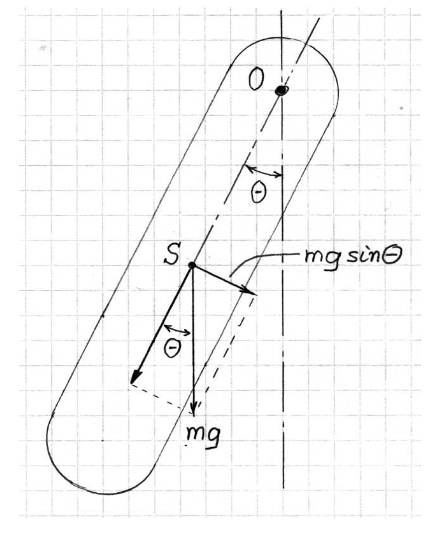
\includegraphics[scale=0.5]{wahadlo.png}
		\caption{Schemat wahadła fizycznego \\ \textit{Źródło: Pracownia Fizyczna WFiIS AGH - ,,Ćwiczenie nr 1 - Wahadła fizyczne"}}
		\label{wahadlo}
	\end{figure}
\newpage

	\begin{figure}[!h]
		\centering
		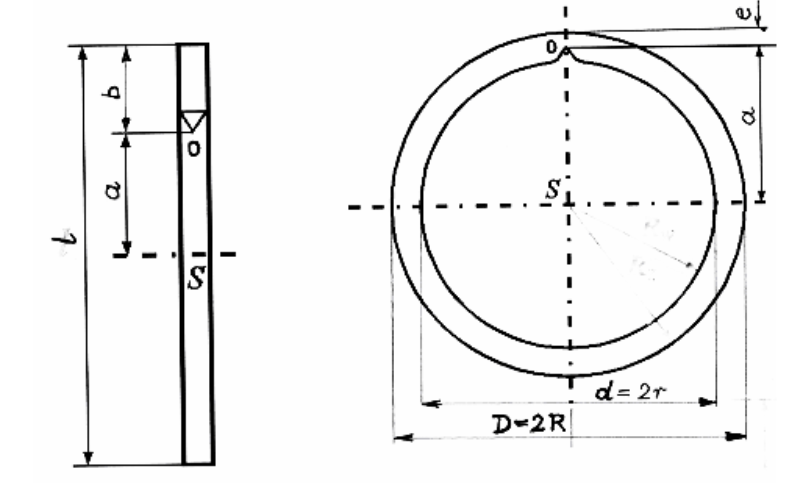
\includegraphics[scale=0.4]{ciala.png}
		\caption{\centering Schemat badanych brył - pręta oraz pierścienia \\ \textit{Źródło: Pracownia Fizyczna WFiIS AGH - ,,Ćwiczenie nr 1 - Wahadła fizyczne"} }
		\label{ciala}
	\end{figure}

%----------------------------------------------------------

	\section{Opracowanie wyników}
	
	\subsection{Pręt}
	
	Zmierzone wielkości masy i długości pręta przedstawione w tabeli 1.
	
		\begin{table}[!h]
		\centering
		\begin{tabular}{ | c | c | c | }
			\hline
			\textrm{Wielkość} & \textrm{Wartość} & \textrm{Niepewność} \\ \hline
			$m$ [g] & 659 & 1  \\ \hline
			$l$ [mm] & 740 & 1  \\ \hline
			$b$ [mm] & 99 & 1  \\ \hline
			$a$ [mm]& 271 & 1  \\ \hline

		\end{tabular}
		\caption{Pomiary masy i długości pręta.}
		\label{Tabela1}	
	\end{table}
	
	Zmierzone wielkości okresu drgań dla pręta zapisano w tabeli 2.
	
	\begin{table}[!h]
		\centering
		\begin{tabular}{ | c | c | c | c | }
			\hline
			\textrm{Lp.} & \textrm{Liczba okresów } k & \textrm{czas } t \textrm{ dla } k \textrm{ okresów [s]} & \textrm{okres } $T_i= \frac{t}{k}$ \textrm{~[s]} \\ \hline
			1 & 10 & 12.86 & 1.286 \\ \hline
			2 & 10 & 12.78 & 1.278 \\ \hline
			3 & 10 & 13.06 & 1.306 \\ \hline
			4 & 10 & 13.15 & 1.315 \\ \hline
			5 & 20 & 26.36 & 1.318 \\ \hline
			6 & 30 & 39.41 & 1.314 \\ \hline
			7 & 10 & 13.18 & 1.318 \\ \hline
			8 & 20 & 26.36 & 1.318 \\ \hline
			9 & 30 & 39.38 & 1.313 \\ \hline
			10 & 10 & 13.12 & 1.312 \\ \hline
		\end{tabular}
		\caption{Pomiar okresu drgań pręta.}
		\label{Tabela2}	
	\end{table}
	
	\flushleft Wartość średnia okresu drgań prętu $T_{p}$ wyliczona na podstawie zmierzonych wartości z tabeli 2: $$T_{1} = 1.308$$
	
	\flushleft Zakładamy, że wartość przyspieszenia Ziemskiego $g = 9.81$.
	
	\flushleft Obliczamy moment bezwładności $I_0$ względem rzeczywistej osi obrotu pręta korzystając ze wzoru na okres drgań:
	$$I_{0_1} = \frac{m \cdot g \cdot a \cdot T^2}{4 \pi^2} = \frac{0.659 \cdot 9.81 \cdot 0.271 \cdot 1.308^2}{4 \pi^2} = 0.076 \textrm{ [kg $\cdot$ m$^2$]}$$ 
	
	\flushleft Korzystając z twierdzenia Steiner'a obliczamy $I_S$:
	$$I_{S_1} = I_0 - m \cdot a^2 = 0.076 - 0.659 \cdot 0.271^2 = 0.028 \textrm{ [kg $\cdot$ m$^2$]}$$
	
	\flushleft Obliczamy moment bezwładności geometrycznie ze wzoru:
	$$I_{S_1}^{(geom)} = \frac{m \cdot l^2}{12} = \frac{0.629 \cdot 0.74^2}{12} = 0.029 \textrm{ [kg $\cdot$ m$^2$]}$$ 
	
	\subsection{Niepewności dla pomiarów pręta}
	
	\begin{itemize}
		\item 
		Niepewność $u(I_{0_1})$:
		$$\frac{u(I_o)}{I_0}=\sqrt{\left (\frac{u(m)}{m}\right ) ^2+\left ( \frac{u(a)}{a}\right )^2+\left (2 \frac{u(T_0)}{T_0}\right )^2} = 0.0043 \textrm{ [kg $\cdot$ m$^2$]}$$
		
		Stąd otrzymujemy: $u(I_0) = 0.00033$ [kg $\cdot$ m$^2$]
		
		\item 
		Niepewność $u(I_S)$:
		$$u(I_S) = \sqrt{(u(I_0))^2 + (a^2u(m))^2 + (-2amu(m))^2} = 0.00057 \textrm{ [kg $\cdot$ m$^2$]}$$
		
		\item 
		Niepewność $u(I_S^{(geom)})$:
		$$u(I_S^{(geom)}) = \sqrt{\left (\frac{l^2}{12} \cdot u(m) \right)^2 + \left (\frac{2lm}{12} \cdot u(l) \right)^2} = 0.00093 \textrm{ [kg $\cdot$ m$^2$]}$$
	\end{itemize}
	
	%-------------------------------------------------
	
	\newpage
	\subsection{Pierścień}

	Zmierzone wielkości okresu drgań dla pierścienia zapisano w tabeli 3.
	
		\begin{table}[!h]
		\centering
		\begin{tabular}{ | c | c | c | }
			\hline
			\textrm{Wielkość} & \textrm{Wartość} & \textrm{Niepewność} \\ \hline
			$m$ [g] & 1360 & 1  \\ \hline
			$D_w$ [mm] & 246 & 1  \\ \hline
			$D_z$ [mm] & 279 & 1  \\ \hline
			$R_w$ [mm]& 132 & 1  \\ \hline
			$R_z$ [mm]& 139.5 & 1  \\ \hline
			$e$ [mm]& 9.7 & 0.05  \\ \hline
			$a$ [mm]& 129.8 & 1  \\ \hline
			
		\end{tabular}
		\caption{Pomiary masy i długości pierścienia.}
		\label{Tabela1}	
	\end{table}
	
	Zmierzone wielkości okresu drgań dla pierścienia zapisano w tabeli 4.
	
	\begin{table}[!h]
		\centering
		\begin{tabular}{ | c | c | c | c | }
			\hline
			\textrm{Lp.} & \textrm{Liczba okresów } k & \textrm{czas } t \textrm{ dla } k \textrm{ okresów [s]} & \textrm{okres } $T_i= \frac{t}{k}$ \textrm{~[s]} \\ \hline
			1 & 10 & 10.21 & 1.021 \\ \hline
			2 & 20 & 20.53 & 1.026 \\ \hline
			3 & 30 & 30.87 & 1.029 \\ \hline
			4 & 40 & 41.10 & 1.028 \\ \hline
			5 & 50 & 51.51 & 1.0302 \\ \hline
			6 & 60 & 61.79 & 1.029 \\ \hline
			7 & 70 & 72.08 & 1.029 \\ \hline
			8 & 80 & 82.36 & 1.029 \\ \hline
			9 & 90 & 92.73 & 1.0303 \\ \hline
			10 & 100 & 103.03 & 1.0303 \\ \hline
		\end{tabular}
		\caption{Pomiar okresu drgań pierścienia.}
		\label{Tabela4}	
	\end{table}
	
	\flushleft Wartość średnia okresu drgań pierścienia $T_{p}$ wyliczona na podstawie zmierzonych wartości z tabeli 4: $$T_{2} = 1.028$$
	
	\flushleft Obliczamy moment bezwładności $I_0$ względem rzeczywistej osi obrotu pierścienia korzystając ze wzoru na okres drgań:
	$$I_{0_2} = \frac{m \cdot g \cdot a \cdot T^2}{4 \pi^2} = \frac{1.36 \cdot 9.81 \cdot 0.1298 \cdot 1.028^2}{4 \pi^2} = 0.046 \textrm{ [kg $\cdot$ m$^2$]}$$ 
	
	\flushleft Korzystając z twierdzenia Steiner'a obliczamy $I_S$:
	$$I_{S_2} = I_{0_2} - m \cdot a^2 = 0.046 - 1.36 \cdot 0.129^2 = 0.023 \textrm{ [kg $\cdot$ m$^2$]}$$
	
	\flushleft Obliczamy moment bezwładności geometrycznie ze wzoru:
	$$I_{S_2}^{(geom)} = \frac{m \cdot (R^2 + r^2)}{2} = \frac{1.36 \cdot (0.1395^2 + 0.132^2)}{2} = 0.025 \textrm{ [kg $\cdot$ m$^2$]}$$ 

	\subsection{Niepewności dla pomiarów pierścienia}

	\begin{itemize}
		\item 
		Niepewność $u(I_{0_1})$:
		$$\frac{u(I_o)}{I_0}=\sqrt{\left (\frac{u(m)}{m}\right ) ^2+\left ( \frac{u(a)}{a}\right )^2+\left (2 \frac{u(T_0)}{T_0}\right )^2} = 0.00802 \textrm{ [kg $\cdot$ m$^2$]}$$
		
		Stąd otrzymujemy: $u(I_0) = 0.00037$ [kg $\cdot$ m$^2$]
		
		\item 
		Niepewność $u(I_S)$:
		$$u(I_S) = \sqrt{(u(I_0))^2 + (a^2u(m))^2 + (-2amu(m))^2} = 0.00051 \textrm{ [kg $\cdot$ m$^2$]}$$
		
		\item 
		Niepewność $u(I_S^{(geom)})$:
		$$u(I_{s}^{(geom)}) =\sqrt{\left (\frac{R_z^2+R_w^2}{2} \cdot u(m) \right )^2+\left (mR_z \cdot u(R_z) \right )^2+\left (mR_w \cdot u(R_w) \right )^2} = 0.00026 \textrm{ [kg $\cdot$ m$^2$]}$$
	\end{itemize}

	\section{Porównanie wyników końcowych}	
	
	Porównanie wyników (niepewność rozszerzona $k = 2$).
	
	\subsection{Pręt}
	
		\begin{table}[!h]
		\centering
		\begin{tabular}{ | c | c | c | c | }
			\hline
			\textrm{ } & $I_0$ z okresu drgań & $I_S$ z tw. Steiner'a & $I_S$ tablicowe \\ \hline
			Wartość [kg $\cdot$ m$^2$] & 0.076 & 0.028 & 0.029 \\ \hline
			Niepewności [kg $\cdot$ m$^2$] & 0.00033 & 0.00057 & 0.00093 \\ \hline

		\end{tabular}
		\caption{Wartości otrzymane i ich niepewności dla pręta.}
		\label{Tabela5}	
	\end{table}

	Aby sprawdzić, czy wynik zawiera się w niepewności rozszerzonej należy podzielić błąd bezwzględny wyniku przez błąd bezwzględny niepewności pomiarowych. Wynik ten musi być mniejszy od 2, ponieważ korzystamy z niepewności rozszerzonej, gdzie $k = 2$.

	$$\frac{|I_S - I_S^{(geom)}|}{\sqrt{u^2(I_S) + u^2(I_S^{(geom)})}} = 0.91$$
	
	Wyniki uważamy za zgodne, ponieważ $\frac{|I_S - I_S^{(geom)}|}{\sqrt{u^2(I_S) + u^2(I_S^{(geom)})}} < 2$. 
	
	\newpage
	\subsection{Pierścień}
	
	\begin{table}[!h]
		\centering
		\begin{tabular}{ | c | c | c | c | }
			\hline
			\textrm{ } & $I_0$ z okresu drgań & $I_S$ z tw. Steiner'a & $I_S$ tablicowe \\ \hline
			Wartość [kg $\cdot$ m$^2$] & 0.046 & 0.023 & 0.025 \\ \hline
			Niepewności [kg $\cdot$ m$^2$] & 0.00802 & 0.00051 & 0.00026 \\ \hline
			
		\end{tabular}
		\caption{Wartości otrzymane i ich niepewności dla pierścienia.}
		\label{Tabela6}	
	\end{table}	

	Aby sprawdzić, czy wynik zawiera się w niepewności rozszerzonej należy podzielić błąd bezwzględny wyniku przez błąd bezwzględny niepewności pomiarowych. Wynik ten musi być mniejszy od 2, ponieważ korzystamy z niepewności rozszerzonej, gdzie $k = 2$.

	$$\frac{|I_S - I_S^{(geom)}|}{\sqrt{u^2(I_S) + u^2(I_S^{(geom)})}} = 0.35$$

	Wyniki uważamy za zgodne, ponieważ $\frac{|I_S - I_S^{(geom)}|}{\sqrt{u^2(I_S) + u^2(I_S^{(geom)})}} < 2$. 
	
	\section{Wnioski}
	Ćwiczenie pozwoliło wyznaczyć bezwładność ciał dla różnych kształtów obiektów. Wyniki uzyskane doświadczalnie są bardzo bliskie wartościom tablicowym (obliczonym z wzoru na moduł bezwładności ciała), pomimo niedoskonałości kształtów badanych ciał takich jak wcięcia w pierścieniu czy metalowy dodatek do zamocowania ciała do wahadła fizycznego. Dodatkowym czynnikiem wpływającym na delikatną rozbieżność wyników jest refleks osoby mierzącej czas okresu drgań, którego nie potrafimy zmierzyć.
	
 \end{document}